\documentclass[11pt,letterpaper]{article}

%%%%%%%%%%%%%%%%%%%%%%%%%%%%%%%%%%%%%%%%%%%%%%%%%%%%%%%%%%%%%%%%%%%%%%%%%
\pagestyle{plain}                                                      %%
%%%%%%%%%% EXACT 1in MARGINS %%%%%%%                                   %%
\setlength{\textwidth}{6.5in}     %%                                   %%
\setlength{\oddsidemargin}{0in}   %% (It is recommended that you       %%
\setlength{\evensidemargin}{0in}  %%  not change these parameters,     %%
\setlength{\textheight}{8.5in}    %%  at the risk of having your       %%
\setlength{\topmargin}{0in}       %%  proposal dismissed on the basis  %%
\setlength{\headheight}{0in}      %%  of incorrect formatting!!!)      %%
\setlength{\headsep}{0in}         %%                                   %%
\setlength{\footskip}{.5in}       %%                                   %%
%%%%%%%%%%%%%%%%%%%%%%%%%%%%%%%%%%%%                                   %%
\newcommand{\required}[1]{\section*{\hfil #1\hfil}}                    %%
\renewcommand{\refname}{\hfil References Cited\hfil}                   %%
%\bibliographystyle{plain}                                              %%
%%%%%%%%%%%%%%%%%%%%%%%%%%%%%%%%%%%%%%%%%%%%%%%%%%%%%%%%%%%%%%%%%%%%%%%%%

\usepackage[utf8]{inputenc}
\usepackage[english]{babel}
\usepackage[compact]{titlesec}
    \titlespacing{\section}{0pt}{2ex}{1ex}
    \titlespacing{\subsection}{0pt}{1ex}{0ex}
    \titlespacing{\subsubsection}{0pt}{0.5ex}{0ex}
    
%Import the natbib package and sets a bibliography  and citation styles
\usepackage{natbib}
\bibliographystyle{abbrvnat}
%\setcitestyle{authoryear,open={((},close={))}}

\usepackage{booktabs} % For formal tables
\usepackage[ruled]{algorithm2e} % For algorithms

% User added packages
\usepackage{caption}
\usepackage{csquotes}
\usepackage{wrapfig}
\usepackage{multirow}
\usepackage{tcolorbox}
\usepackage{todonotes}
\usepackage{graphicx}
\usepackage[table,xcdraw]{xcolor}
%\documentclass[xcolor=table]{beamer}
% \usepackage{subcaption} % for subfigures
\usepackage{colortbl}
\usepackage[shortlabels]{enumitem}
\setlist{noitemsep}
\setlist[1]{labelindent=0} % < Usually a good idea
\setlist[itemize]{leftmargin=0}
\setlist[itemize]{label=\textbullet}
%\setlist[itemize][label=\textbullet]
%[label=\emph{\alph*})]
\setlist[itemize]{labelindent=0}
\setlist[itemize]{itemindent=0}
\setlist[enumerate]{labelsep=*, leftmargin=1pc}
\setlist[enumerate,1]{label = \arabic*.,
ref = \arabic*}
\setlist[enumerate,2]{label = \emph{\alph*}),
ref = \theenumi.\emph{\alph*}}
\setlist[enumerate,3]{label = \roman*),
ref = \theenumii.\roman*}
\setlist[description]{font=\sffamily\bfseries}


\newenvironment{WrapText}[1][r]
  {\wrapfigure{#1}{0.5\textwidth}\tcolorbox}
  {\endtcolorbox\endwrapfigure}
  
\newcommand{\cmu}[1]{%{\bf XX if we include CMU data:} \textcolor{blue}{#1}
}

% User-Defined Commands
\newcommand{\fig}[1]{Figure~\ref{#1}}
\newcommand{\tbl}[1]{Table~\ref{#1}}
\newcommand{\algo}[1]{Algorithm~\ref{#1}}
\newcommand{\sect}[1]{Section~\ref{#1}}
\newcommand{\etal}[0]{ et al.~}
\newcommand{\eg}[0]{{\em e.g.,~}}
\newcommand{\ie}[0]{{\em i.e.,~}}
\newcommand{\etc}[0]{{\em etc.~}}

\newcommand\numparticipants[0]{209 }
\newcommand\numdiscriminationevents[0]{454 }
\newcommand\numdiscriminationeventsfinal[0]{448 }


\newcommand\acomment[1]{\textcolor{orange}{\textit{Anind: #1}}}
\newcommand\anind[1]{\textcolor{orange}{\textit{Anind: #1}}}
\newcommand\sandy[1]{\textcolor{purple}{\textit{Sandy: #1}}}
\newcommand\jen[1]{\textcolor{red}{\textit{Jen: #1}}}
\newcommand\eve[1]{\textcolor{pink}{\textit{Eve: #1}}}
\newcommand\jm[2]{\textcolor{blue}{#1}\textcolor{red}{\textit{Jen: #2}}}
%\newcommand\jen[2]{\textcolor{blue}{#1}\textcolor{red}{\textit{Jen: #2}}}
%\newcommand\jen[2]{\textcolor{blue}{#1}\textcolor{red}{\textit{Jen: #2}}}
\newcommand\ycomment[1]{\textcolor{blue}{\textit{Yasaman: #1}}}
\newcommand\yasaman[1]{\textcolor{blue}{\textit{Yasaman: #1}}}
\newcommand\kcomment[1]{\textcolor{brown}{\textit{Kevin: #1}}}
\newcommand\kevin[1]{\textcolor{brown}{\textit{Kevin: #1}}}
\newcommand\pcomment[1]{\textcolor{green}{\textit{Paula: #1}}}
\newcommand\paula[1]{\textcolor{green}{\textit{Paula: #1}}}

% Document starts
\begin{document}
% Title portion
\title{Addressing Sources of Stress for Women and Underrepresented Minorities in STEM Learning Environments }


\setcounter{page}{1}
%\include{NSFdata}

%%%%%%%%% SUMMARY -- 1 page, third person
% e.g:  "The PI will prove" not "I will prove"

\required{Project Summary}
% This should be a brief statement of the problem you plan to address.
% It should look something like an abstract. 

\required{Intellectual Merit}
% This is why your project is interesting and will help further
% knowledge in the field of mathematics. 

\required{Broader Impacts}
% There are 4 kinds of broader impacts.
% 1. advance discovery and understanding while promoting teaching,
% training and learning
% 2. broaden the participation of underrepresented groups
% 3. disseminated broadly to enhance scientific and technological
% understanding
% 4. benefits of the proposed activity to society
 \setcounter{page}{1}

\section{Introduction}
\label{sec:intro}

 
Engineering is a challenging discipline to study, and doubly so for students from groups that are underrepresented in engineering, who deal with discrimination, bias, microaggressions, and other forms of “othering” during their careers. These groups include racial and ethnic minorities (\eg \cite{Mcgee:2011}), women (\eg \cite{Moss-Racusin:2012}), LGBTQIA+ identifying students (\eg \cite{Cech:2011}) and first-generation college students (\eg \cite{Pascarella:2004,Carrigan, et al., 2019}. These challenges can be compounded when multiple of these identities come into play (\eg \citep{Williams:2014}). Despite significant funding and attention paid to diversity in engineering, the percentage of B.S. degrees awarded to women in 2017 was just 21.3\%.  This is even more distressing because 21.3\% was a 10-year high \citep{Asee 2017}. 

 
Although the experiences of minority populations have been studied for some time now, this is a very challenging problem to make progress on. It can be particularly difficult to effectively measure the impact of problems, and of solutions, on students. This is work that typically must be very specific and focused. For example, take the question of bias against women. It can be difficult to prove that bias exists, and is caused by gender, but in the case of resume assessments, a clever way to measure bias is to vary the name (and nothing else) in a resume. Using this approach, multiple studies have demonstrated bias in assessment of resumes based on presumed gender. In one recent double-blind study, 127 faculty in biology and physics each reviewed an undergraduate resume with a randomly assigned female or male name for a fictional lab manager position \citep{Moss-Racusin:2012}. Men were rated as being more competent, hireable, and worthy of mentoring and higher pay than women. Reviewer gender, seniority, field, and age had no effect on outcome. An earlier psychology study of 238 faculty who received four gender-randomized resumes showed similar outcomes \citep{Steinpreis:1999}. Still, the impact of those biases is hard to measure, especially since they are often small and may take years to add up. However, the impact of small differences in the evaluation of female candidates of 1-5\% (a purported degree to which gender bias affects performance ratings \citep{Barrett:1993}) can be used to simulate how discrimination will impact gender distributions over time in an organization \citep{Martell:1996}, as well as productivity \citep{Cole:1991}. In simulation, such differences accumulate, leading to approximately a 2:1 difference in measures of success between men and women at the most senior levels \citep{Cole:1991,Martell:1996}. 
%More recently, a study in 2014 showed that in an online course, female instructors are given lower student evaluations of teaching than males, if students believe that they're female.  This occurs {\it even if the instructor is actually a male.} This study took place in an introductory course in anthropology/sociology, a field that has a much higher population of female students than engineering \cite{MacNell:2014}.  
%% Here is the ref: L. MacNell, A. Driscoll, and A. N. Hunt.  What's in %%a name: exposing gender bias in student ratings of teaching. %%{\Innovative Higher Education}, 40(4): 291-303, 2014. 

At the end of decades of work, we have a model (though no field test) of impact, and still no solution -- no field-tested technique for reducing this bias, or its impact. And this body of work was focused almost entirely on resume assessment of women, just a small piece of the bigger picture for minority students attempting to succeed in their fields. How, then, can we expect to solve these problems? We argue that what is needed is a far more comprehensive approach to data collection. In the era of big data, a comprehensive change in the way that we collect and assess the college student experience is possible. We can  move from the lab to the field,  connect action to behavior, and  collect longitudinal data. This in turn makes it possible to understand bias in  new ways.  

There is past literature that demonstrates that large-scale longitudinal data collection can help us to understand depression and other mental health factors and how they relate to student outcomes (\eg \cite{wang2014studentlife}). That study depended on occasional survey questions combined with a large amount of passive data collection. By complementing self reports with passive data collection we can use big data to create an image of behavior, while learning about specific challenges that students face through self reports. This ability to connect behavior to experience, in the field, is what past studies lack.  %information about discrimination and bias in the filed that can help us understand it better. 

The technological innovations needed to make this possible are here -- we have access to devices that can passively capture many of the activities that students engage in; and technical approaches that can actively capture the remainder of the information we need to know. This is an exciting era for data collection and analysis and one in which it becomes possible to study issues such as discrimination and bias, at scale and in real-time, and truly understand their impact. This important information will help support the design of effective interventions, policy, and decision making to improve the experiences of not just diverse students in engineering, but all students in engineering. 
 
These insights led us to raise seed money necessary to launch a pilot study with 200 students a year ago. Since then, we have revised our study protocol to further improve it, completed the initial analysis presented in this proposal, and begun year one of data collection with 200 first year students. In both the pilot study and year one, we worked hard to ensure a representative sample of underrepresented groups in engineering (UREs), as shown in Table~\ref{tab:study-participants}. This includes women, underrepresented minorities, first-generation college students, and LGBTQ students. 
While we are still collecting year one data as of this writing, our pilot data shows high compliance and the importance of the rich and varied data that we collect for understanding discrimination: Ninety-one participants from the pilot reported almost 450 separate instances of discrimination and we are able to demonstrate the impact of these experiences on sleep and phone use and connect this to emotional state.  \paula{}
%Our  data show that all of these groups are at risk for discrimination and other obstacles that may impact retention. Further, we argue that an intersectional approach is critical to understanding the challenges these groups face. Thus, we consider discrimination, harassment, and other challenges together with a range of identities in a single holistic study.  

Our proposal is to follow as many of the 200 students from year one as possible for three more years, so that we can truly understand the impact of discrimination on engineering students’ experiences and success. While the data from year one can help to shed light on short term impacts of discrimination, it is only with four years of data that we can learn about important long term impacts such as retention. 

\subsection{Intellectual Merit}
\label{sec:questions}

Our proposed work will leverage the collected data to help improve our theoretical understanding of the impact of discrimination on students; answer important questions about both short and long term impacts of discrimination; shed light on mediating factors such as micro-climates and resilience; and ultimately support intervention design. We  propose to test a model of the student experience (shown in Figure~\ref{fig:model} ) that we believe helps to capture the differential stressors experienced by women and other minorities in engineering in a way that can ultimately be quantified and operationalized. 

As shown in Figure~\ref{fig:model}, and described in more depth in Section~\ref{sec:back}, much is known about the relationship between discrimination and long term stress outcomes such as physical and mental health. (\eg \cite{Ong:2009}). However there are also a number of open questions which will be the focus of our work. These are shown in Figure~\ref{fig:model} in the boxes with dashed lines along the dashed arrows. There are four primary questions that we hope to answer. Here we talk about each and explain why it is important. 

\begin{figure}
    \centering
    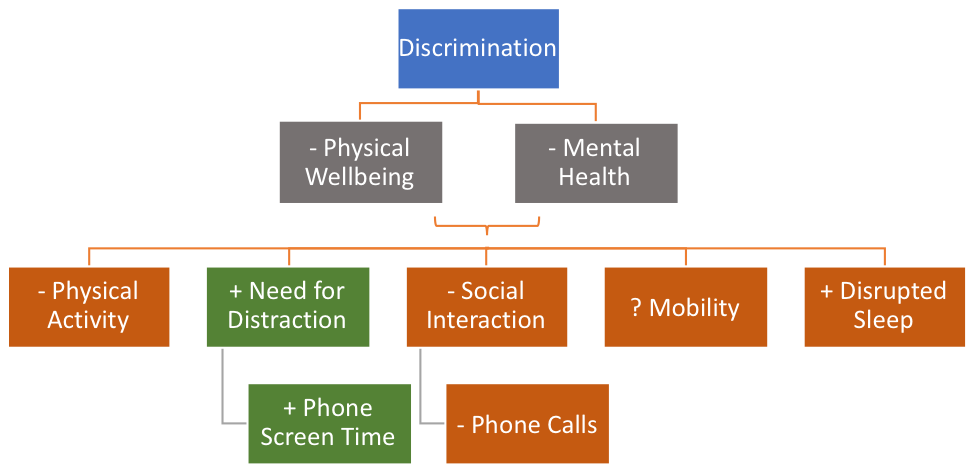
\includegraphics[width=12cm]{img/model.png}
    \caption{Theoretical model relating student experiences to long term outcomes.}
    \label{fig:model}
\end{figure}


\paragraph{Daily Discrimination $\rightarrow$ Short Term Behavior} Our pilot study has already found almost 450 separate instances of  \textit{daily discrimination}, alongside which we have extensive passively collected behavioral data, unlike any former study. Thus, our first research questions ask what we can learn about the impact of daily discrimination from behavioral data. This is particularly important in an educational context where we may find, for example, that discrimination is both more likely at high stress times (such as midterms) and more impactful (if students lose sleep and are thus less well prepared). T
\begin{enumerate}[start=1,label={\bfseries RQ\arabic*}, leftmargin=1cm]
    \item \label{itm:rq-behavior} What is the impact of daily discrimination on short term behaviors? We hypothesize that this is similar to stress, which leads to a second question:
    \item \label{itm:rq-behavior-size} Can we quantify the size of any behavior change due to a daily discrimination event, and the length of time it will last? 
    \item \label{itm:rq-severity-impact} How does the severity of discrimination change these outcomes?
\end{enumerate}

\paragraph{Short Term Behavior $\rightarrow$ Long Term Outcomes} Our second set of questions follow from the first, by extending it to a longitudinal data set. While the impact of discrimination on long term outcomes is something that has been studied, no prior data set has been able to relate short term and long term impacts as ours can. 
\begin{enumerate}[start=4,label={\bfseries RQ\arabic*}, leftmargin=1cm]
    \item \label{itm:rq-short-long} Which long-term outcomes are linked to short-term behavior changes and to what degree?
    \item \label{itm:rq-which-long} Are there specific short term changes that are more likely to relate to long term impacts than others?
    \item \label{itm:rq-severity-long} Are there specific factors such as cumulative severity of discrimination or number of repetitions that predict long term impacts?
\end{enumerate}
 
 \paragraph{Micro-Climates $\rightarrow$ Indirect Impact} Although novel intervention design is out of scope for this proposal, it is our hope that the proposed work will help us to understand the impact of existing micro-climates, which can in turn guide intervention design. We have already identified multiple micro-climates that may impact the discrimination-stress process highlighted in Figure~\ref{fig:model} including STARS, the introductory course sequence the student takes, and participation in SEEEDS mentoring (all are defined in Sidebar~\ref{sidebar:definitions}). We believe that these micro-climates will indirectly impact outcomes through their impact on mediating factors and the likelihood of daily discrimination events. 
 
\begin{WrapText}
\begin{description}[leftmargin=1cm]
\item[STARS] paragraph about STARS
\item[Introductory Sequence] The introductory course experience can have a big impact on the likelihood of discrimination due to the level of competitiveness...
\item[SEEEDS mentoring]
\item[FIGS?]
\end{description}
\end{WrapText}

\begin{enumerate}[start=7,label={\bfseries RQ\arabic*}, leftmargin=1cm]
    \item \label{itm:mc-daily-discrimination} Which micro-climates will reduce exposure to daily discrimination? Which micro-climates will increase exposure?
    \item \label{itm:mc-internal-mediators} Which micro-climates will increase or decrease mediating factors such as resilience and two-way social support? Will this translate into different short-term or long-term behavior outcomes?
    \item \label{itm:mc-external-mediators} Which micro-climates will increase or decrease external mediating factors such as exposure to negative events? Will this translate into different short-term or long-term behavioral outcomes?
\end{enumerate}
 
The contributions of our work will include (1) a more complete theoretical model of the impact of discrimination than previous works
  Our work will also make it possible (2) to document, for the first time, \textit{what behaviors change and in what ways} following acts of discrimination and (3) to demonstrate, for the first time, \textit{which micro-climates reduce that impact} and through what mechanisms. Finally (4) This in turn can guide the development of interventions that help to mediate or reduce the experience of discrimination.
Our goal is to develop a holistic understanding of the impacts of discrimination on the participation and retention of UREs over their college career. 

\subsection{Broader Impact}
\noindent
Our proposed work will improve outcomes for UREs by (1) quantifying impact of unfair treatment (discrimination, harassment and so on)  on students (2) demonstrating to what degree discrimination impacts success and retention of underserved groups (3) quantifying the protective impact of a deployed intervention, an intentionally-created micro-climate targeted at the most at-risk students in Engineering and Computer Science. 

The University of Washington is one of 8 or 10 large flagship public universities in the country. The student experiences in these different settings are likely to be similar in terms of program scale and the range of students and student backgrounds entering the engineering program. This makes it likely that similar interventions will work in similar ways. The impact of discrimination on mental health and physical health is already well-demonstrated in multiple studies. Thus, we expect that our findings will translate to similar large public universities, meaning that we have the potential to impact X 1000 engineers in training each year. We hope that our work will translate to other universities engineering programs working to increase their diversity as well. 

In addition, we will disseminate the results of our proposed work to other universities who are working to retain underserved students in Engineering and Computer Science.  Co-PI Riskin is PI of the UW STARS program, which was founded at UW and Washington State University in 2013,  STARS is an adaptation of the Goldshirt Program at the University of Colorado, Boulder, which is entering its 11th year. Through UW’s leadership, the redshirt model has since been adopted at three additional institutions through a six-institution Redshirt in Engineering Consortium grant from the National Science Foundation (UW, WSU, University of Colorado, Boulder, University of Illinois, Urbana-Champaign, Boise State University, and University of California, San Diego). Through the Redshirt Consortium, UW is engaged in sharing best practices in supporting students from first-generation and low-income backgrounds. 

In the remainder of this proposal, we describe the pilot study that we have already conducted and present some simple preliminary analysis of the data demonstrating promise that our approach can indeed support investigation of these research questions.
 
\subsection{Team}
 
Jennifer Mankoff is the Richard E. Ladner professor in the Paul G. Allen School of Computer Science and Engineering. She has been working with under-represented populations for over a decade (\eg \cite{newman2004perceptions,DBLP:conf/huc/DillahuntMPF09,DBLP:conf/cscw/DillahuntM14,DBLP:conf/huc/DillahuntMP10,DBLP:journals/pacmhci/EarlyHHRWM18,DBLP:conf/chi/OLearyZMR19}). In addition, she has led this study effort at the University of Washington (UW), helped to create the team, and will continue to lead the effort over the remaining years of the study. Her background in Human Computer Interaction has prepared her well to run this effort and her research includes a mix of qualitative behavioral work (\eg \cite{DBLP:conf/huc/DillahuntMPF09,DBLP:conf/chi/MankoffKKRW11}), mixed methods/quantitative behavioral work (\eg \cite{DBLP:conf/ph/CrawfordGSAM14,DBLP:journals/pacmhci/EarlyHHRWM18}), and technical work in behavior modeling (\eg \cite{DBLP:conf/chi/BanovicBCMD16}). 
 
Eve Riskin is Professor of Electrical and Computer Engineering, Associate Dean of Diversity \& Access in the UW College of Engineering, and founder of the UW STARS program.  She is also Faculty Director of UW's ADVANCE program and has been working on diversity and inclusion in engineering for nearly two decades.  She  has published extensively on diversity in engineering education (e.g. EVE-FILL-IN-HERE ).
 
Paula Nurius discrimination

\section{Background and Related Work}
\label{sec:back}

\label{sec:back-discrimination}
\noindent 
Discrimination, defined as adverse behaviors, negative judgment, or unfair treatment towards a person, is an uncontrollable and unpredictable stressor, and as such severely influences health and well-being \citep{Williams:2009}. However, there are also risk and protective factors that can explain why similar experiences impact people differently \citep{SeridoAlmeidaWethington:2004}.

The impact of discrimination, in terms of the response it elicits and  health outcomes, can thus be studied within a general stress and coping framework \citep{Pearlin:1999}. 
Ong \etal (\citeyear{Ong:2009}) apply this framework to  study  response to incidents of discrimination, using it to account for the variability in different people's stress responses based on the previous and current context of their life. They developed a theoretical model relating chronic and daily exposure to discrimination to stress based on Pearlin \etal's stress and coping framework \citep{Pearlin:1999}. In a  study of  174 African American doctoral students they demonstrated the relationship between both chronic and daily discrimination to distress, and show that chronic exposure to discrimination exacerbates reaction to daily discrimination incidents (but not other negative events). Since then, other works have demonstrated a clear relationship between discrimination and stress (\eg \cite{Pieterse:2007}). 
Because of discrimination's links to stress, it is not surprising that it can impact both physical and psychological wellbeing, as summarized next:

\paragraph{Physical Well-being:}
\label{sec:back-discrimination-physical}
When discrimination triggers physiological stress responses it can cause
(\eg heightened blood pressure, heart rate, and cortisol secretions \citep{Brondolo:2008, Steffen:2003, Smart:2010}), which can lead to serious conditions such as heart disease (\eg \cite{Marshall:1997, Cohen:1994}). Should it happen repeatedly, discrimination increases reactivitity to stressful situations \citep{GuyllMatthewsBrom-berger:2001} and weakens the body's protective resources, thus increasing the risk of illness similar to other forms of cumulative stress \citep{GeeSpencerChenTakeuchi:2007}. Additionally, discrimination is directly correlated with more unhealthy behavior (\eg smoking, drinking, substance use \citep{LandrineKlonoff:1996, MartinTuchRoman:2003}). 

\paragraph{Psychological Well-being:}
\label{sec:back-discrimination-mental}
The association between exposure to discrimination and mental health is well supported by empirical evidence \citep{Pascoe:2009} as well as large scale population studies \citep{Kessler:1999}. Not only is discrimination directly associated with higher levels of depression, anxiety, and psychological distress in general, it is negatively correlated with identifiers of healthy psyche such as positive affect \citep{Schmitt:2014}. The magnitude of the associations is larger for negative health outcomes (\eg depression \citep{Schmitt:2014}) and is comparable to major stressors such as sexual assault or combat experience \citep{Kessler:1999}. 
Consistent with Ong \etal's (\citeyear{Ong:2009}) application of the stress and coping framework to discrimination, responses are different depending on things like prior exposure  \citep{Kessler:1999}. 

\subsection{Open Questions}
\noindent The relationships documented in the literature are summarized in Figure~\ref{fig:model}. Although there is a great deal of evidence that both daily and cumulative discrimination are linked to stress, and thus impact both physical and psychological wellbeing.  However, a unified model that relates short term behavior to long term outcomes is still lacking. Although Ong \etal (\citeyear{Ong:2009}) propose multiple models, their work focused only on self reported measures. In addition, it is not yet clear how discrimination relates specifically to academic outcomes such as grades and retention. Finally, no prior work has quantified the impact of risk factors and protective factors on these relationships. 
A better understanding of the relationship between short term changes and long term outcomes can help us to design better interventions and improve our ability to model the overall effects of discrimination.
\section{Proposed Study}
\label{sec:study}
\noindent We propose a four-year study that follows 200 students from their first year in the College of Engineering through graduation. Participants in this study will provide massive amounts of raw behavioral data supplemented with survey data that leverages standard scales for measuring mediating factors, exposure to discrimination, and mental and physical health. In addition, participants will provide bi-weekly experience sampling surveys  (EMAs) to answer questions about daily discrimination, daily negative events, and daily changes in anxiety and stress. Details of our approach  follow.

Over the last two years, we have designed, refined, and tested our measures; collected pilot data from 174 students in January-June of 2018; and launched the first year of data collection for the proposed study in April of 2019, with 200 first-year engineers.  Based on compliance with the pilot (which was highest during the first quarter), our plan for future years is to run the study for one quarter per year, and additionally to answer questions about exposure to discrimination and negative events for the entire year.  

Our 2018 pilot study demonstrates the viability and power of our method, both in terms of our ability to collect useful data from participants with high compliance, and our ability to connect that data to interesting results. Our preliminary analysis found that over half (91) of students experienced discrimination, and those students reported 448 distinct incidents. These incidents were associated with reduced sleep, more time on the phone, and changes in physical activity (\ref{itm:rq-behavior}), which lasted 1-2 days after the event (\ref{itm:rq-behavior-size}, as described in Section~\ref{sec:result}. These results are the first to quantify the type, size, and duration of the impact of daily discrimination events on short term behavior. Our study is the first to deploy technology capable of gathering the data necessary to study these types of things.  

We refer to our pilot study throughout this section to illustrate the viability of our approach. However, our primary goal in this section is to document our proposed method. 

\subsection{Method}
\noindent
We propose to collect data from 150 University of Washington Engineering students over four years. This will allow us to study students' experience in a challenging and critical period of their lives. Four years of data is necessary to track long-term changes (an important part of our model) and collecting it is the only way to get a complete picture of factors like retention in major.
Extending the study to four years is feasible within the proposal period  since we are already engaged in year-one data collection.

We expect some attrition, and this is reflected in the budget. However, we hope to have at least 90 students still participating by the end of the study based on our pilot study's retention rate, which was approximately $85\%$. Thus, if we start with 150 students, we expect 132 in year two, 110 in year three, and 92 in year four. \paula{need here or elsewhere to present power analysis? This is a pretty low number for assessment of longitudinal changes and trends.}


\subsubsection{Participants}
\label{sec:study-participants}
We have over-sampled from underrepresented groups in engineering (UREs), including women (gender discrimination is an ongoing problem \cite{johnson2018sexual}), underrepresented minorities (URMs) such as Latinx, African American and Native American students, and first-generation students.  We propose to use snowball sampling and targeted emails to reach our population of interest. \paula{anything more needed to support this sampling strategy? issues of representativeness?}

In addition, we sampled from specific micro-climates of interest (such as STARS), again using targeted emails to reach populations of interest.

We illustrate our ability to recruit a representative sample by summarizing our pilot population in Table~tbl{tab:study-participants}. Note that our pilot study did not focus on engineers. Our year one deployment has already begun, and while we have not completed analysis as of this writing, it has been similarly successful, with participants including $48\%$ women, $14\%$ URMs and half of this year's STARS cohort.  \paula{do we need here more details about micro-climates given that this far we have only noted two and need to more fully define what these are?}

\begin{table}[]
\small
\begin{tabular}{l|c|c|c|c|}
\cline{2-5}
& \multicolumn{2}{c|}{\begin{tabular}[c]{@{}c@{}}  \textbf{Completed Pilot}\end{tabular}} & \multicolumn{2}{c|}{\begin{tabular}[c]{@{}c@{}} \textbf{Dropped Out of Pilot}\end{tabular}} \\ 
\cline{2-5} 
& \textbf{All (N=176)} & \textbf{Engineers (N=73)} & \textbf{All (N=33)} & \textbf{Engineers (N=11)} \\ 
\hline
\multicolumn{1}{|l|}{Women (64\%)} & 114 (54\%) & 41 (20\%) & 19 (9\%) & 7 (3\%)  \\
\hline
\multicolumn{1}{|l|}{\begin{tabular}[c]{@{}l@{}}URM (12\%) \end{tabular}} & 18 (9\%) & 15 (7\%) & 10 (5\%) & 5 (2\%) \\ \hline
\multicolumn{1}{|l|}{First-Generation Students} & 51 (24\%) & 27 (13\%) & 11  (5\%) & 7 (3\%)  \\ \hline
\multicolumn{1}{|l|}{LGBTQIA+ (12\%)} & XX & XX & XXX & XX  \\
\hline 
\end{tabular}
\caption[Pilot - sample breakdown]{Sample breakdown of gender and minority status in our pilot study. Categories are non-independent. Of the 33 who dropped out, 13 did so before the break between quarters, and 20 before post \sandy{"post-quarter"?} questionnaires. URM refers to under-represented minorities (i.e., students who are African-American, Native American, Latinx, and Pacific Islander).
}
\label{tab:study-participants}
\end{table}


\jen{need \%age of first gen students and percentagis for LGBTQIA+}

\subsubsection{Surveys}
Study participants will answer hour-long written questionnaires about their life experiences, self regulation and coping skills, and health behaviors before and after the study (i.e., \textit{pre} and \textit{post} surveys).  They will also fill out twice weekly surveys about their affect, stress, and experiences of unfair treatment (Experiential Momentary Assessment (EMA) surveys).  For two weeks, we will send EMA surveys four times a day to get more detailed information. A summary of survey and EMA measures is shown in Table~\ref{tab:study-surveys}.

Concerns with a study of this intensity are compliance and retention. To help ensure both, we propose to stay in frequent touch with participants and to pay them well for their participation.  Of 209 participants in the pilot study, 176 (84\%)  completed the post-study questionnaire. The  compliance rate for EMA surveys was 85\%. These very high rates give us confidence in the viability of the study method. 

\begin{table}[]
\smaller
\begin{tabular}{p{1.5mm}|p{2.9cm}|l|p{9.3cm}|}
\cline{2-4}
 & \textbf{Measure}   & \textbf{Administration} & \textbf{Scales / Items Included in the Measure} \\ \hline
\multicolumn{1}{|c|}{\multirow{4}{*}{\vspace{-7mm}\rotatebox[origin=c]{90}{Pre or Post}}} & Social Experiences or Perceptions & pre, post & UCLA Loneliness (loneliness) [Russell \citeyear{Russell:1996}], 2-way SSS (social support) [Shakespeare-Finch \citeyear{Shakespeare:2011}]  \\ \cline{2-4} 
\multicolumn{1}{|c|}{} & \multirow{2}{*}{Stress \& Coping} & pre, post & MAAS [Brown, \citeyear{Brown:2003}], ERQ  (emotion regulation) [Gross \citeyear{Gross:2003}], PSS (stress) [Cohen \citeyear{Cohen:1983stress}], BRS  (resilience) [Smith \citeyear{Smith:2008}] \\ \cline{2-4} 
\multicolumn{1}{|c|}{} & Physical \& Mental Health% and Sleep 
& pre, post  & CHIPS [Cohen \citeyear{Cohen:1983positive}] (physical health), CES-D (depression) [Radloff \citeyear{Radloff:1977}], %RSQ \cite{Armey:2009}, 
STAI (anxiety) [Kabacoff \citeyear{Kabacoff:1997}]%, PSQI \cite{Buysse:1989} 
\\ \hline%\cline{2-4} 
\multicolumn{1}{|c|}{\multirow{6}{*}{\vspace{-7mm} \rotatebox[origin=c]{90}{EMA}}} & \multirow{2}{*}{Affect} & daily, weekly & Feeling anxious, depressed, frustrated, overwhelmed, lonely, happy and connected on a scale of 1 (not at all) to 5 (extremely) \\ \cline{2-4} 
\multicolumn{1}{|c|}{} & \multirow{2}{*}{\textit{Unfair Treatment\dag}} %(exposure \& severity) 
& daily, weekly & Unfairly treated because of ancestry or national origins, gender, sexual orientation, intelligence, major, learning disability, education or income level, age, religion, physical disability, height, weight or other aspect of one's physical appearance\\ \hline
\end{tabular}
\caption{Proposed measures in pre- or post-study questionnaires and EMA surveys. The high-level construct related to each measure is shown in parentheses after the acronym. Our proposed measure of daily discrimination is italicized and marked with a cross (\dag). Other scales provide information about context and mediating factors. 
}
\label{tab:study-surveys}
\end{table}


\paragraph{Proposed use of survey data to populate theoretical model.} 
The survey data is the source of our most important \textit{primary stressor} variable, daily discrimination. Participants are asked about this twice-weekly, as follows: ``Did you experience unfair treatment for any of the following reasons?'' A range of reasons will be provided, including gender, race, \etc We will also ask about severity, possible reasons for unfair treatment, and which type of person was responsible (\eg peer, teacher). This will provide the basis, source, and severity for the primary stressor in the model in Figure~\ref{fig:model}.

We will use this data to calculate two additional measures:  \textit{exposure} (any report of unfair treatment qualifies) and \textit{severity} (ratio of total reports to total available responses, \ie number of times the question was answered over the course of the study). 

Survey data will also be used to measure \textit{mediating factors}, including resilience, social support, chronic discrimination and negative events (left-most box in Figure~\ref{fig:model}). We propose to use a  \textit{pre/post} scale that asks about discrimination over the lifetime, year, and quarter, along with other negative events. We also use standard, well-tested psychological scales to measure factors like Resilience and Social Support (see Table~\ref{tab:study-surveys}). 

\textit{Long-term behavior outcomes} will come from a combination of survey data about mental and physical health (as assessed at the end of the study) and institutional data provided by the university (we have access to data about grades and retention). \textit{Context} will come from survey data.

\subsubsection{Short-Term Behavior Data}
We will collect short-term behavior data (orange box on right side of model in Figure~\ref{fig:model}\sandy{I don't see this on figure 1}) using a combination of custom phone software and a Fitbit. We propose to give participants a Fitbit~Flex~2, which records the number of steps taken and per-minute sleep status (\eg asleep or awake). The phone software we will use is the AWARE Framework \cite{Ferreira:2015}. AWARE has been tested in many studies, including our own pilot study, and provides an excellent, stable option for such studies. It can collect a wide range of passive data, including  
location; phone screen status; call logs for incoming, outgoing and missed calls; and activity information (\eg walking, running, or still) inferred by the phone. 
\tbl{tab:study-sensors} summarizes the sensors we propose to collect and proposed details of their collection (\eg sampling rate) based on what we learned in our pilot study. 

\paragraph{Proposed use of short-term behavior data.} We propose to operationalize the short-term behavior data, as summarized in Table~\ref{tab:study-sensors}.  We will extract behavior features using  the AWARE feature extraction library \citep{Chikersal:2019}. We calculate features daily and for four different parts of the day: night (12am-6am), morning (6am-12pm), afternoon (12pm-6pm), and evening (6pm-12am) in an approach modeled on \citep{wang2014studentlife}'s study, which connected behavior to stress on a similar data set. 

We will group the features into the five categories that the literature suggests are relevant to stress (see below). \paula{there are other behaviors more or additionally linked to stress such as substance use, social media, etc. The table below includes passive data. Is there value in noting here that we are also including self-report behavioral data?} We focus on stress literature because of the lack of information about which of these behaviors will be impacted by  exposure to discrimination. However, since discrimination is known to  adversely affect mental and physical health, and to cause distress (\eg \cite{Ong:2009}), focusing on stress-related behaviors makes sense as a starting place. Our pilot data analysis provides further evidence for this choice, as described in Section~\ref{sec:result}.

\begin{description}
\item[Physical Activity.]     Higher levels of physical activity are correlated with fewer symptoms of anxiety and depression \citep{Stephens:1988}, as well as lower levels of emotional distress \citep{Steptoe:1996}. Moreover, past work on mobile health sensing has successfully used features based on inferred activity, \eg to predict depression in students \citep{Wang:2018} or relapse in schizophrenic patients \citep{Wang:2016}. 
\item[Phone Usage.] Distraction, an emotion-regulation strategy to reduce distress and negative feelings \citep{Sheppes:2011}, can manifest itself in the form of excessive or purposeless phone screen time. In fact, phone screen overuse is linked to depression and anxiety in college students \citep{Demirci:2015}. Encouragingly, patterns of phone screen time, particularly in relation to location of use, have been previously used as depression symptoms \citep{Wang:2018}. \paula{only below is it clear that phone usage means screen only, not calling--see if I got this right}
\item[Social Interaction.] Social support and interaction are key to psychological health and well-being \citep{Kawachi:2001}. Unsurprisingly, mental health problems, such as depression, are inversely related to quality and quantity of social interactions \citep{Nezlek:1994}. Moreover, social-support seeking is a common strategy people use to cope with distress \citep{Carver:1997}.  In terms of social context, previous research has used information on nearby Bluetooth devices (\eg \cite{wang2014studentlife}), which can potentially encompass friendship information as suggested in \citep{Eagle:2009}. Social interactions have been used as indicators of mental health \citep{Wang:2016}.  \paula{so soc interactions are info about calls only, yes? does it pick up texting? emailing, etc?}
Discriminatory encounters can initially lead to increased calls as people seek support. However, when depressive symptoms increase, social participation might drop (\eg social withdrawal \citep{Girard:2014}) . 
\item[Mobility.] Mental health conditions, such as depression or anxiety, that are characterized by avoidance behaviors can potentially impact mobility patterns. \paula{provide more info about what "variety of activities" means in Table 3; this will help distinguish mobility and activity and the differing interpretations of these data} There is indeed evidence connecting people's mobility to the severity of depressive symptoms \citep{Saeb:2015, Saeb:2016} and their levels of anxiety \citep{Huang:2016}. 
\item[Sleep.] There is significant comorbidity between sleep problems and a number of mental health complications, including depression \citep{Vandeputte:2003}, anxiety \citep{Morrison:1992}, and malconduct \citep{Papadimitriou:2005}. Sleep detection using wearable and mobile sensors has been the topic of mobile health research (\eg \cite{Min:2014}), and sleep monitors are commercially available, \eg through Fitbit. In relation to mobile sensing of mental health, \citet{wang2014studentlife} and \citet{Wang:2018} have used measures of sleep to model academic performance and levels of depression in college students. 
\end{description}

\vspace{1em}
\noindent
To summarize, the behaviors that we might expect based on the literature include reduced physical activity, increased phone screen time, reduced phone calls, reduced mobility, and increased sleep disruptions. These five areas of potential behavior change form the basis for our features, which are summarized in Table~\ref{tab:study-sensors}.

\begin{table}[]
\centering
\smaller
\begin{tabular}{|l|l|l|l|p{5.5cm}|}
\hline
\textbf{Relevant Behavior}         & \textbf{Sensor} & \textbf{Source}        & \textbf{Sampling}            & \textbf{Information Collected}                                                 \\ \hline
\multirow{2}{*}{Physical Activity} & Step            & Fitbit                 & 1 sample per min             & Number of steps                                                                \\ \cline{2-5} 
                                   & Activity        & \multirow{4}{*}{AWARE} & 1 sample per 5 min           & Type of activity: walking, running, on bicycle, in vehicle, still, unknown     \\ \cline{1-2} \cline{4-5} 
\multirow{2}{*}{Phone Usage}                        & Screen          &                        & \multirow{2}{*}{event-based} & Screen status (locked, unlocked, off, and on) events                           \\ \cline{1-2} \cline{5-5} 
\multirow{2}{*}{Social Interactions} & Call            &                        &                              & Time and duration of incoming, outgoing, and missed calls                      \\ \cline{1-2} \cline{4-5} 
\multirow{2}{*}{Mobility}               & Location        &                        & 1 sample per 10 min          & GPS latitude, longitude, altitude                                              \\ \cline{2-2} \cline{4-5}
& Activity & & 1 sample per 5 min & Variety of activities \\ \hline
%Mobility               & Location        &                        & 1 sample per 10 min          & GPS latitude, longitude, altitude\\ \hline
\multirow{2}{*}{Sleep }                             & Sleep           & Fitbit                 & 1 sample per min             & Duration and onset of sleep, minutes to fall sleep, of awake, and after wakeup \\ \hline
\end{tabular}

\caption[Sensors]{Sensor data collected by AWARE and used in our analysis.}
\label{tab:study-sensors}
\end{table}

\section{Initial Results from Pilot Study}
\label{sec:result}

\begin{wrapfigure}{l}{0.5\textwidth}
\vspace{-1.5em}
    \centering
    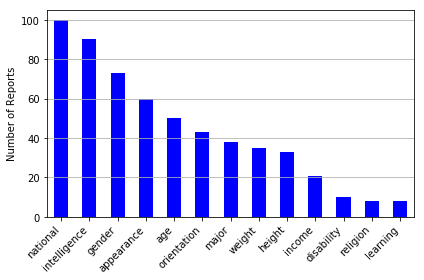
\includegraphics[width=3.3in]{img/discrimination_breakdown.png}
`    \caption[Unfair treatment type breakdown]{Breakdown of \numdiscriminationeventsfinal reports of unfair treatment by type. \textit{National}, \textit{Orientation}, and \textit{Learning} refer to ancestry or national origin, sexual orientation, and learning disability, respectively. See \tbl{tab:study-surveys} for details of all categories. Participants could report multiple types of unfair treatment in each incident report.
}
    \label{fig:data-discrimination-breakdown}
\end{wrapfigure}

To further demonstrate the viability of our approach, we present a preliminary analysis of one part of the model, shown in Figure~\ref{fig:model}. The model is based on our pilot data, which included only first-year students from both engineering and non-engineering majors, as shown in Table~\ref{tab:study-participants}. 

\noindent For this analysis, we focused on answering aspects of \ref{itm:rq-behavior} (the impact of daily discrimination on short-term behaviors) and \ref{itm:rq-behavior-size} (the size and length of behavior change). 

\paragraph{Analysis Approach.}
We use hierarchical linear modeling (HLM) for this analysis. HLM is an extension of linear regression for units (\eg individuals, schools, communities) with correlated/common features. %We use a two-level model in which individual participants, who were repeatedly sampled over time, are clustered within themselves.
%HLM allows for flexibility in how change over time is modeled such that these models can fit discontinuous and non-linear changes. Additionally, 
HLM models do not require individuals to report the same number of observations over time and thus can handle an unequal number of observations per person and uneven spacing between observations (\cite{maas2005sufficient}).

Considering the inter-related nature of the variables and their sheer numbers, along with the small number of participants in the pilot study, the behavior features considered as outcomes must be reduced to avoid an excessive number of comparisons that increase the chance of type I error (false positive). 

Prior to analysis, we used feature selection to reduce the size of the feature space. We selected the top five metrics (when available) for each sensor for further analysis. Much more can be said about analysis, a domain in which PI Mankoff is innovating (\eg \cite{DBLP:conf/huc/EarlyFM16,DBLP:conf/chi/BanovicBCMD16,DBLP:conf/huc/KoehlerBOMD14}). Although not a focus of this proposal, that research and expertise will be leveraged where useful to improve upon this proposed work.

\paragraph{Prevalence of daily discrimination.}
Our pilot study data lacked information about race-related discrimination, an approach we corrected in the year one deployment. However, it included discrimination on the basis of a range of other variables, such as ancestry/national origin, intelligence, and gender (the three most common) to religion, learning, and disability (the three least common); (see \fig{fig:data-discrimination-breakdown}). Participants reported \numdiscriminationeventsfinal distinct incidents of unfair treatment during the pilot study. \fig{fig:data-discrimination-breakdown} shows the prevalence and breakdown of these reports by category. We found that unfair treatment was more prevalent among women: 73\% of all reports of unfair treatment were reports from women. Contrary to our expectations, unfair treatment was equally prevalent in both engineering and non-engineering majors. \paula{consider saying what all the non students are re disciplines?}


\paragraph{\ref{itm:rq-behavior} Impact of daily discrimination on short-term behavior.} We found short-term impacts of discrimination on mental health and behavior. Discriminatory encounters showed strong (high-confidence) relationships with same-day depression and frustration (\textit{p} $<.001$), but no strong relationships with change in positive affect. This is consistent with earlier reports that discrimination is more strongly associated with higher negative but not lower positive states \citep{Schmitt:2014}. Changes in depression and frustration are illustrated in Figure~\ref{fig:results-affect-dieoff}.  \eve{Need a figure label to refer to here.}

We also found a relationship with behavior, particularly behaviors relating to sleep, activities, steps, and phone use \paula{this meaning screen use only or also calls? are the differences in theorized directions?}, which all differed significantly from the baseline on the day of discrimination. This supports our theoretical model, which links discrimination to stress and thus predicts changes in stress-related behaviors. 

\paragraph{\ref{itm:rq-behavior-size} Size and length of short-term behavior change.}

Because we chose to use regression modeling, we could easily quantify the impact of the changes found in ~\ref{itm:rq-behavior}. We found that people walked more (by $\sim$500 steps), had more evening calls ($\sim$1 more), interacted more with their phone in the morning ($\sim$5 more interactions), and spent less time in bed ($\sim$15 minutes less), when they have experienced discrimination in the last day. 

To model the change in impact over time, we examined exposure to discrimination on the day of (day 0) and response variables (health and behavior) on day 1, day 2, etc. and calculated whether there was a significant difference as compared to people who reported no daily discrimination.  We found that discriminatory encounters showed strong (high-confidence) relationships with same-day and next-day daily reports of depression and frustration. 

These changes in affect also translated into changes in behavior. To relate them to behavior, we examined six of the most predictive variables found in our analysis. Our results (shown in Figure~\ref{fig:die-off}) demonstrate that most, if not all, of the impact found in our data occurred on  day 0 (day of the discrimination). This effect then declined (\textit{p}-values rise) over the next two days. \paula{is there value in looking at the relationship of chronic discrim or negative events perhaps cumulatively with daily discrim to assess if effects last longer for those with greater prior stress load? this is part of what we have set up in the intro. May decide not to do here but it likely will be important to see trends for those with greater chronicity of stress histories. might add to section below re social support}
%The effect size is also stronger on the day of unfair treatment than the day after (larger $\beta$'s). After that, this distress returns to values similar to those in the control group (people who did not report unfair treatment).

\paragraph{\ref{itm:rq-short-long} Which long-term outcomes are linked to short-term behavior changes?}
Although we lack sufficient longitudinal data to fully analyze this research question (since the pilot data encompasses less than one year of the student experience), we can explore the link between behavior change and mental health. 

We used the same modeling approach to study the impact of mediating factors on the link between short-term behavior change and long-term outcomes. Although the immediate impact of singular instances of unfair treatment faded quickly, people who reported unfair treatment \textit{and} scored lower on social support, reported higher levels of depression at the end of the study ($\beta$ = -0.15, p-value=0.027). This is predicted by the literature  (\eg \cite{Mossakowski:2014}) and aligned with our theoretical model: having social support buffers some of the psychological distress of daily discrimination, and reduces the likelihood that it will impact long-term outcomes.

\begin{figure}
     \centering

% \begin{subfigure}[t]{0.49\textwidth}
% %    \small
%     \centering
%     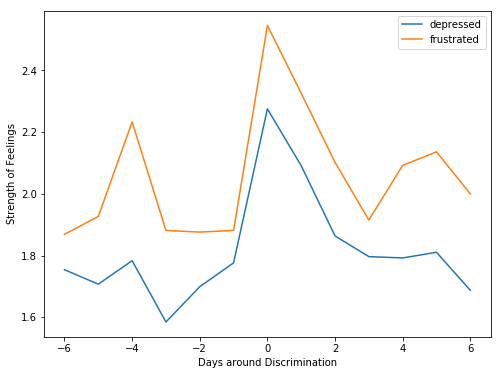
\includegraphics[width=\textwidth]{img/affect-beforeafter.png}
%     \caption[Affect ratings before and after unfair treatment]{Ratings of feeling depressed and frustrated (1: not at all, 5: extremely) 3 days before and 3 days after reports of unfair treatment. The day of unfair treatment is at zero. Note the large peak on the day of the report, which lasts an additional day but then subsides.
%     }
%     \label{fig:reeults-affect-dieoff}
% \end{subfigure}
% % \hfill
% \begin{subfigure}[t]{0.49\textwidth}
%     \centering
    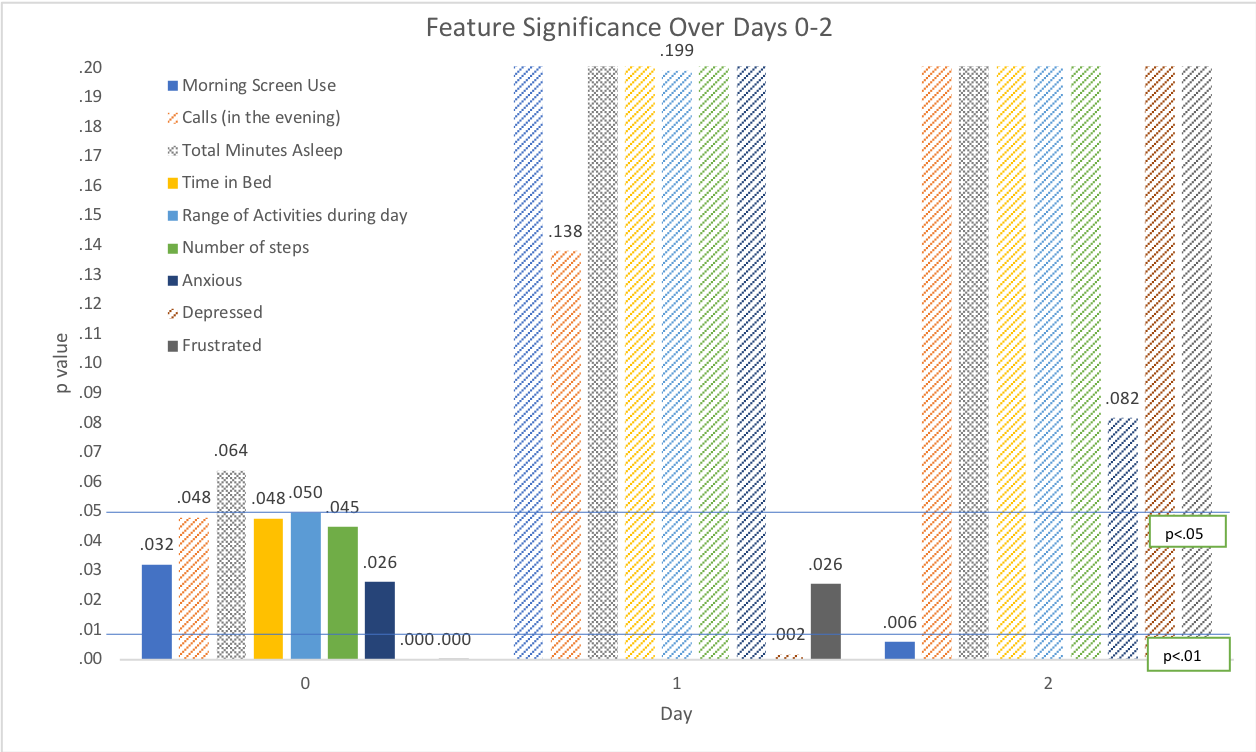
\includegraphics[width=\textwidth]{img/feature-significance}
    \caption[Feature significance over time]{Patterns of feature significance within two days of the discrimination event. The shortest bars represent the highest significance values (\eg Depressed and Frustrated on day 0; Depressed on day 1; Morning screen use on day 2). Most short-term relationships appear on the day of the event and a few on the day after.  Lines are shown at p$<.05$ and p$<.01$.\\ }
    \label{fig:die-off}
% \end{subfigure}

\end{figure}


%\paragraph{Impact of microclimate and other moderators on unfair treatment:} \jen{xx to fill out. There was very old data in the proposal}
%In the chart below, the Y axis shows the percentage of engineers who were at risk on each scale in January (start of study) and June (end of study) of 2018. We choose to focus on engineers in order to compare engineers enrolled in protective micro-climates from their peers who do not share the same protective factors. These micro-climates are the Direct Admit program, in which students are directly admitted to the major and do not have to compete for admission to an engineering department; and the STARS program, which is an onboarding program for first-generation college students, and students from low-income backgrounds and high-poverty high schools in Washington; these students tend to struggle in engineering programs because they  might not be fully prepared for their prerequisite  courses. 

\section{Planned Analyses as Data Is Collected}

Although discrimination is the target of our study, it must be explored in the context of all of the hardships faced by students (and their reactions to the hardships). In our model, this is represented in the form of mediating factors. In our analysis, this also needs to accounted for.

\subsection{\ref{itm:rq-behavior}: The Impact of Discrimination on Short-term Behavior}

 Framing: Which Behaviors? How long? How Severe?
 
 Over the course of the proposed study, we expect to collect approximately 1,800 examples of discrimination from which we can derive information about short- term behavior changes. From a statistical and machine learning perspective, this should be more than sufficient to support strong conclusions with respect to \ref{itm:rq-behavior} \ref{itm:rq-behavior-size} and \ref{itm:rq-severity-impact}.

\subsubsection{Measures} The outcome measures we will use to study \ref{itm:rq-behavior} are behaviors, time, and size of behavior change. The first of these outcome measures is by design focused on features of behavior that can be passively captured (as described in \ref{sec:??}, these are extracted from mobile phone sensors). 

\subsection{Analytic approach}
We are proposing hierarchical multiple regression, which was applied already in our pilot analysis with success. Because of the intersectional nature of our data (i.e. someone may both be a woman, and a person of color; or be engaged in multiple micro-climates), we will need to do repeated analysis focusing on specific sub-populations and factors. 


\subsection{The impact of discrimination on long term behavior}
In the case of long-

term outcomes, our sample size will be approximately 150 (depending on attrition). This is still a sufficient sample size to explore questions such as \ref{itm:rq-short-long}, \ref{itm:rq-which-long} and \ref{itm:rq-severity-long} using outcome measures such as retention in major and GPA and analytic techniques such as regression. 

\subsection{The impact of micro-climates on the overall response to discrimination}
Finally, there is the question of how micro-climates impact students. This is the most exploratory aspect of our study. Micro-climate variations will by the nature of our study only impact small groups of students (such as the \XXFILLIN students in STARS in our year-one cohort). To assess the impact of micro-climates, we will need to move beyond statistical techniques to combine qualitative analysis and quantitative analysis. This will allow us to identify and then look for trends over time using regression to assess how students are impacted, or to identify common themes that might be found outside of those micro-climates, allowing us to increase our sample size.

Although this aspect of the proposed analysis is less well-defined, we are confident that our mixed-methods approach will result in rich data that will be able to inform intervention and suggest valuable future work. This study is part of a much larger effort, as evidenced by the involvement of STARS leadership, and we plan to capitalize on that larger momentum to ensure that our work seeds the next steps needed to fully explore the impact of micro-climates. 

The micro-climates we will focus on include STARS, SEEEDS, FIGS, and the Major status. The first is expected based on existing studies of it to have a very positive impact on students, including their likelihood of exposure to discrimination and response to it. The second and third are less rigorous programs, that share certain overlap with STARS. By comparing these we may learn about what aspects of STARS are necessary to its success, and whether those aspects can translate into less time-intensive, more scalable programs effectively. Finally, the major status, specifically competitive effort to join the major (which currently accepts only X\% of students who apply) is likely to have a negative impact on students. 

\subsection{Risks}
One challenge for our analysis is the size of our study. Although we plan to pursue funding to expand the sample size, as of this writing, the proposed sample size is approximately 200. Although this is somewhat limiting, we are confident that in the case of short term behavior, our sample will be much larger. This is because, 



While this is smaller than in the case of short-term behavior, our expectation based on pilot data is that approximately half of the sample will experience some discrimination, and approximately a quarter will experience repeated discrimination. In addition, based on studies of computer science departments such as the Taulbee report, \cite{} it would be normal to expect attrition rates of X\% for men and Y\% for women, which might be attributable to discrimination experiences. 




%\section{Proposed work: Increasing the Specificity and Robustness of Analysis}
The pilot work just shown is exciting and compelling, but it is not sufficient to solve the problems this proposal sets out to address. 



\subsection{Diving Deeper into the data}
%\paragraph{Interviews about Discrimination:} 
In addition, there are specific topics that require follow up data collection. For example, we propose to conduct interviews that can help to enrich our understanding of students’ experience of unfair treatment. These interviews will in turn guide both quantitative data analysis and further refinements to our data collection procedures. We are currently refining an interview protocol based on pilot interviews as well as our reading of the literature. We hope these interviews will help to answer several questions that can guide our data analysis including:
What reactions do students remember having? How does this relate to what we observe in the data itself? 
What stakeholders and settings are most important to understanding the experience of discrimination? 
Answers to these questions can guide (1) what we focus on quantifying in the data analysis (2) how social science researchers who study discrimination might want to design their study protocols to capture key facets of discrimination.


\subsection{Intervention}
It is our goal not only to describe the student experience, but also to help improve it. Thus, starting in year two of this proposal (years three/four of our data collection) we will start exploring the potential to intervene in the student process through interventions that impact both internal and external factors. Specifically, for internal interventions, we will explore the value of teaching a variety of methods for increasing resilience and other protective factors identified through analysis of the collected data from our pilot study and year one.

For external interventions, we plan to study the impact of STARS in more depth by following a matched sample of students in and not in STARS with similar demographics. We will also work to assess specific things about STARS driven by our research. For example, based on our data about gender, educating students about how to act toward each other, or modifying group membership or training groups to ensure fairer treatment, are both examples of external work that may be able to help address discrimination. These interventions essentially help to create new micro climates that are more protective/supportive. 
%Extended Data Analysis: From Description to Prediction
%Our proposed work has allowed us to capture real-time information about the student experience at scale. Our data analysis goals will operate at several scales (descriptive, analytic, and predictive).

%\subsection{Further analysis of the student experience}
%Descriptive Goals: From a descriptive perspective, our goal is to develop specific descriptive analysis that have immediate value for policy. For example, as we expand our sample over years and across different groups, we should be able to use this to drive answers to questions such as 

%Whether direct admit students benefit more when they reach critical mass (engineering is rapidly increasing the number of direct admit students, so we have a natural experiment in place that lets us compare across years).

Can we differentiate individual versus system differences

Under what circumstances do difficult events cascade into a larger set of troublesome issues for students? In our data, some people seem to bounce back while others don’t. What differentiates these groups of students?

\jen{ say anything about prediction? I'm not sure we have enough analytics for that in this proposal, probably a different proposal?}

%Move from a detection model to a prediction model: The descriptive and analytic goals that we are putting together are contributions in their own right, but taken together they set the scene for something equally important: Predictive work. We have some preliminary evidence that the data supports prediction of things such as increases in depression, XYZ. Some specific goals for prediction:
%Can we predict problems before they occur which can support intervention in the future?
%Can we predict things that are onerous to collect with high enough accuracy that we could reduce the EMAs (e.g. experiences of discrimination)?
%Xxx what else 
%Summarize the importance and impact that prediction could have….


%\input{6-discussion}
\section{Conclusion and Work Plan}
\label{sec:conclusion}
The pilot work just described is exciting and compelling, and it demonstrates the value of our proposed work. First, we are able to verify the most comprehensive model of discrimination and its impact on behavior and outcomes to date. As illustrated in Figure~\ref{fig:model}, we hypothesize that discrimination's impact on mental and physical health will affect those stress-related behaviors (\ref{itm:rq-behavior}). Our study will not only help to test that hypothesis but also to quantify the scope, direction, and longitudinal impact of discrimination on each type of behavior, improving our theoretical model of discrimination's impact on individuals (\ref{itm:rq-behavior-size}, \ref{itm:rq-severity-impact}).
 
 In addition, ours is the first model at this level of detail to tie discrimination specifically to student outcomes, such as GPA and retention. Our model will help to link short-term behavior to long-term outcomes (\ref{itm:rq-short-long}, \ref{itm:rq-which-long}, \ref{itm:rq-which-long}). This makes it extremely valuable for helping with intervention design and policy setting on university campuses.
 For example, the buffering effect of social support has implications for intervention design. 

Lastly, our approach is the first to explore the relationship between specific micro-climates and the mediating factors that help to buffer people from the impact of discrimination (\ref{itm:mc-daily-discrimination}, \ref{itm:mc-internal-mediators}, \ref{itm:mc-external-mediators}). By studying micro-climate impact on outcomes, we can further support intervention design and enrich our theoretical model. 

Educational institutions are characterized by dominant attitudes and behaviors. Some disciplines are particularly vulnerable to gender, race, and nationality bias, including  engineering \cite{sevo2010bias}.  We believe that it is critically important to study these issues in the educational context, a sentiment recently argued in an NSF Dear Colleague Letter encouraging research in sexual harassment and other forms or harassment in STEM contexts.\footnote{\url{www.nsf.gov/pubs/2019/nsf19053/}} The pervasiveness of discrimination experiences in our data surprised even our seasoned team, and addressing them is critical to creating a diverse and informed workforce. This can be accomplished only by shedding light on these darker aspects of engineering education. As Bill and Melinda Gates said in their  recent Annual Letter,\footnote{\url{https://www.gatesnotes.com/2019-Annual-Letter}} data is sexist (and racist), and the biases inherent in the data we collect are necessary, indeed critical, to address. This study is a first attempt to do so, and we intend to contribute to the development of this domain as an important topic of study for computational researchers.   

%A comprehensive change in the way that we study the college student experience. 
%Our research facilitates this thanks to new changes in the ease of capturing real-time student information. Our work is innovative because it allows us to study the student experience at scale, provides before-after data around events such as discrimination,
% quantifies impact, and allow us to design the most effective interventions and policies.
 
Our work plan is as follows: 


%\begin{table}[]
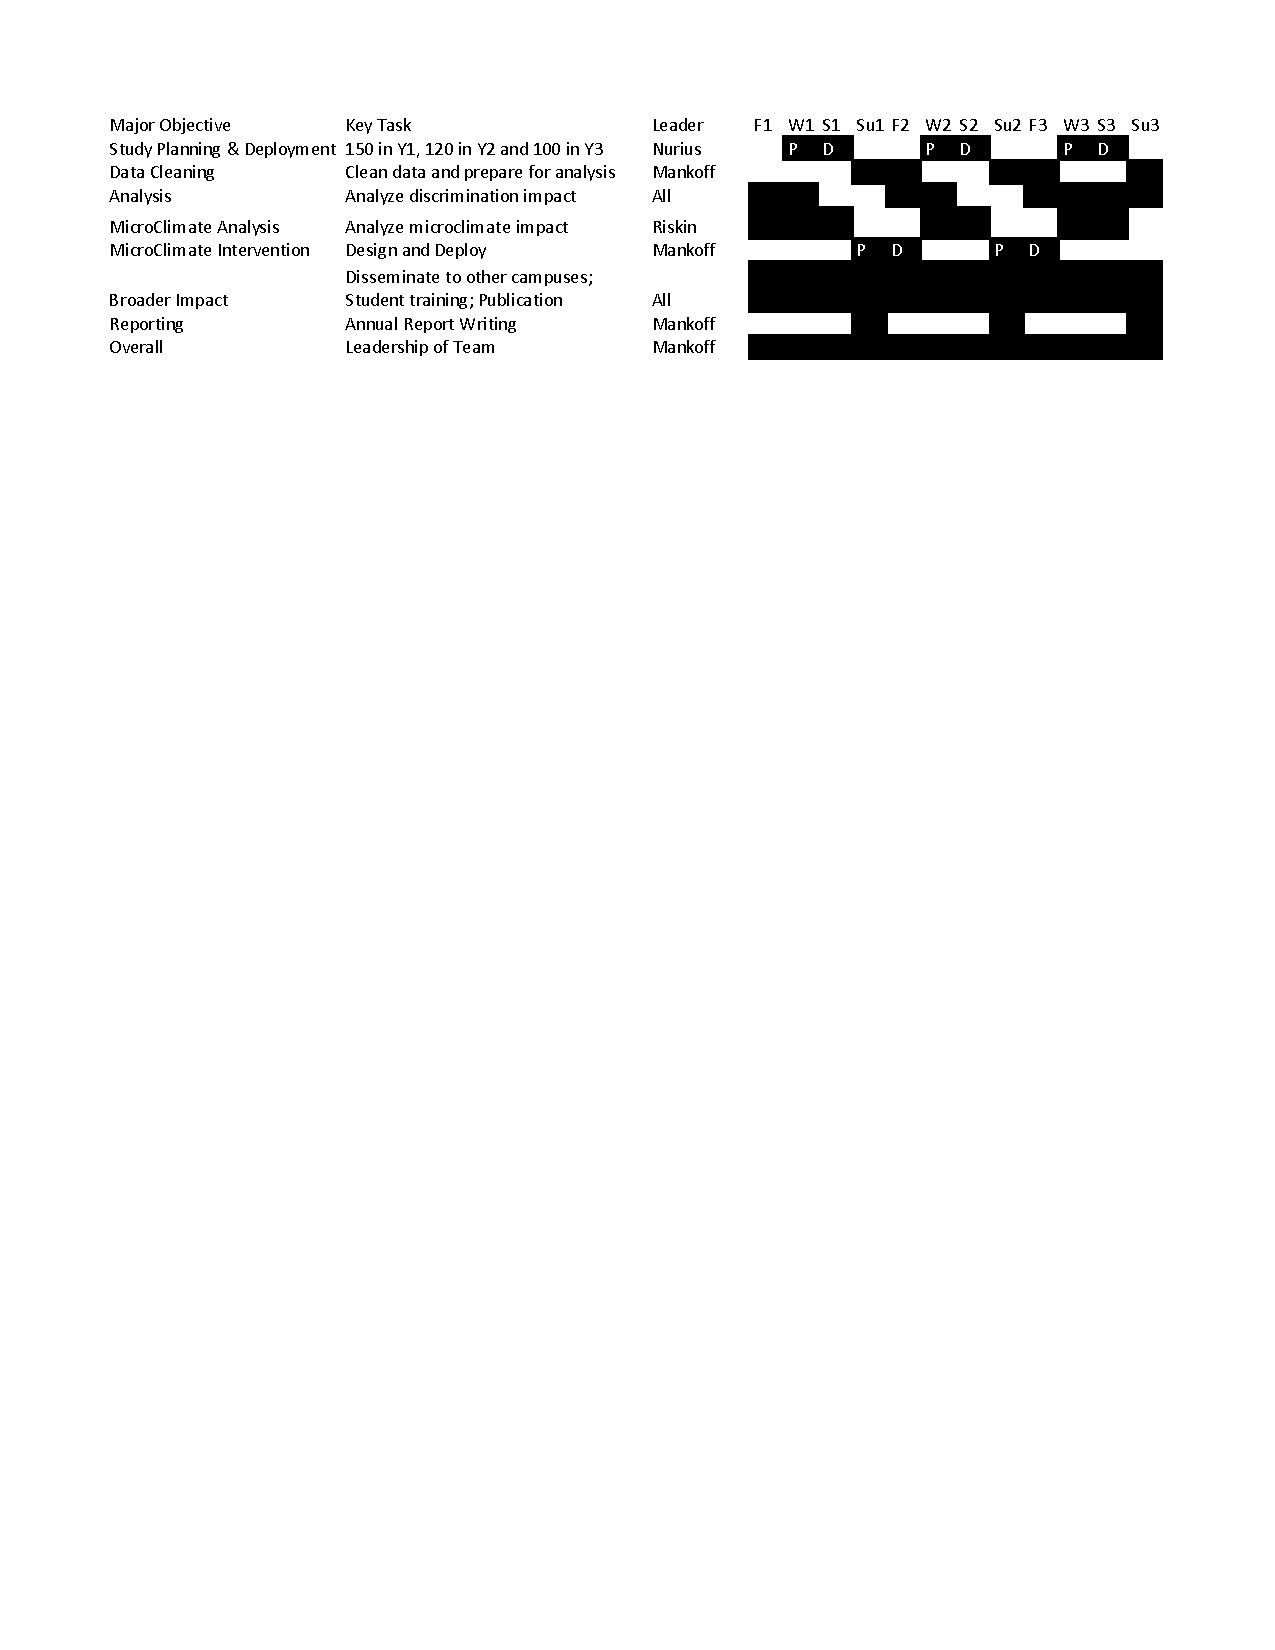
\includegraphics[width=\textwidth]{img/workplan.pdf}
% \small
% \resizebox{\textwidth}{
% \begin{tabular}{p{3cm}p{3cm}lllllllllllll}
% \textbf{Major Objective} &  \textbf{Key Task} & \textbf{Leader} &  F1 &  W1 & S1 & Su1 & F2 & W2 & S2 & Su2 & F3 & W3 & S3 & Su3 \\ \hline
% Study Planning \& Deployment & 150 in Y1, 120 in Y2 and 100 in Y3 & Nurius &  &  P &  D &  &  &  P & D &  &  & P & D &  \\
% Data Cleaning & Clean data and prepare for analysis & Mankoff &  &  &  & X & X &  & X & X &X &  &  & X \\
% Analysis & Analyze discrimination impact & All & X&X&  &  &X& X  &  &  & X & X & X & X\\
% Microclimate Analysis & Analyze microclimate impact & Riskin &X&X & X &  &  & X & X &  &  &X&X &  \\
% Microclimate Intervention & Design and deploy & Mankoff &  &  &  & P & D &  &  &  P &  D &  &  &  \\
% Broader Impact & \begin{tabular}[c]{@{}l@{}}Disseminate to other campuses; \\ Student training; publication\end{tabular} & All &  & X & X & X & X & X & X & X & X & X& X& X& X\\
% Reporting & Annual Report writing & Mankoff &  &  &  & X &  &  &  & X &  &  &  & X \\
% Overall & Team leadership & Mankoff & X & X & X & X & X & X & X & X & X& X& X& X
% \end{tabular}%
% }
%\end{table}

\jen{talk about sample size and how it relates to budget--expected drop-off in participation, why it is sufficient, how we have already gotten seed funding that can help us possibly increase it.}

%%%%%%%%% REFERENCES -- no limit

% this should include only items referenced in the project description
% it is not a bibliography of related reading.

% Each reference must include the names of all authors (in the same
% sequence in which they appear in the publication), the article and 
% journal title, book title, volume number, page numbers, and year of 
% publication. If the document is available electronically, the website 
% address also should be identified


%\bibliographystyle{alpha}
%\bibliography{discrimination.bib}
\bibliographystyle{ACM-Reference-Format}
\bibliography{discrimination}
 \setcounter{page}{1}

\end{document}
